\documentclass{beamer}
\usepackage{booktabs}
\usepackage{array}
\usepackage{ragged2e}
\usepackage{tikz}
\usepackage{tcolorbox}
\usepackage{fontawesome5}
\usepackage{multicol}
\usepackage{xcolor}
\usepackage{colortbl}
\usepackage{graphicx}
\usepackage{adjustbox}
\usepackage{lmodern}
\usepackage[T1]{fontenc}

\usetikzlibrary{shadows.blur, positioning, calc, shapes.geometric}
\tcbuselibrary{skins, breakable}

\newcolumntype{L}[1]{>{\raggedright\let\newline\\\arraybackslash\hspace{0pt}}m{#1}}

% ---------------- THEME ----------------
\usetheme{Madrid}
\usecolortheme{default}

% Custom Colors
\definecolor{primaryblue}{RGB}{30,40,110}
\definecolor{darkblue}{RGB}{15,20,80}
\definecolor{accentblue}{RGB}{60,120,216}
\definecolor{lightgraybg}{RGB}{245,245,248}
\definecolor{cardgray}{RGB}{250,250,252}
\definecolor{accentorange}{RGB}{230,126,34}
\definecolor{accentgreen}{RGB}{39,174,96}
\definecolor{footerblue}{RGB}{45,55,130}
\definecolor{bordergray}{RGB}{170,170,185}
\definecolor{accentred}{RGB}{231,76,60}
\definecolor{accentpurple}{RGB}{142,68,173}
\definecolor{warmyellow}{RGB}{241,196,15}
\definecolor{softcyan}{RGB}{26,188,156}
\definecolor{slidebg}{RGB}{252,252,255}

\setbeamercolor{frametitle}{bg=primaryblue, fg=white}
\setbeamercolor{block title}{bg=primaryblue, fg=white}
\setbeamercolor{block body}{bg=lightgraybg, fg=black}
\setbeamercolor{background canvas}{bg=slidebg}

\setbeamertemplate{navigation symbols}{}
\setbeamertemplate{headline}{}

% ---- Card-style tcolorbox definitions ----
\newtcolorbox{infocard}[2][]{%
  enhanced, colback=white, colframe=accentblue, boxrule=0.4pt,
  arc=6pt, left=6pt, right=6pt, top=4pt, bottom=4pt,
  fonttitle=\bfseries\small\color{white},
  title=#2, coltitle=white, colbacktitle=accentblue,
  attach boxed title to top left={xshift=6pt, yshift=-2.5mm},
  boxed title style={arc=3pt, boxrule=0pt, colback=accentblue},
  shadow={1pt}{-1pt}{0pt}{black!15}, #1
}

\newtcolorbox{alertcard}[2][]{%
  enhanced, colback=accentred!3, colframe=accentred!70, boxrule=0.4pt,
  arc=6pt, left=6pt, right=6pt, top=4pt, bottom=4pt,
  fonttitle=\bfseries\small\color{white},
  title=#2, coltitle=white, colbacktitle=accentred!85,
  attach boxed title to top left={xshift=6pt, yshift=-2.5mm},
  boxed title style={arc=3pt, boxrule=0pt, colback=accentred!85},
  shadow={1pt}{-1pt}{0pt}{black!12}, #1
}

\newtcolorbox{successcard}[2][]{%
  enhanced, colback=accentgreen!3, colframe=accentgreen!60, boxrule=0.4pt,
  arc=6pt, left=6pt, right=6pt, top=4pt, bottom=4pt,
  fonttitle=\bfseries\small\color{white},
  title=#2, coltitle=white, colbacktitle=accentgreen!80,
  attach boxed title to top left={xshift=6pt, yshift=-2.5mm},
  boxed title style={arc=3pt, boxrule=0pt, colback=accentgreen!80},
  shadow={1pt}{-1pt}{0pt}{black!12}, #1
}

\newtcolorbox{purplecard}[2][]{%
  enhanced, colback=accentpurple!3, colframe=accentpurple!50, boxrule=0.4pt,
  arc=6pt, left=6pt, right=6pt, top=4pt, bottom=4pt,
  fonttitle=\bfseries\small\color{white},
  title=#2, coltitle=white, colbacktitle=accentpurple!80,
  attach boxed title to top left={xshift=6pt, yshift=-2.5mm},
  boxed title style={arc=3pt, boxrule=0pt, colback=accentpurple!80},
  shadow={1pt}{-1pt}{0pt}{black!12}, #1
}

\newtcolorbox{orangecard}[2][]{%
  enhanced, colback=accentorange!3, colframe=accentorange!50, boxrule=0.4pt,
  arc=6pt, left=6pt, right=6pt, top=4pt, bottom=4pt,
  fonttitle=\bfseries\small\color{white},
  title=#2, coltitle=white, colbacktitle=accentorange!85,
  attach boxed title to top left={xshift=6pt, yshift=-2.5mm},
  boxed title style={arc=3pt, boxrule=0pt, colback=accentorange!85},
  shadow={1pt}{-1pt}{0pt}{black!12}, #1
}

% Stat box (small pill-shaped card)
\newcommand{\statbox}[3]{%
  \begin{tcolorbox}[enhanced, colback=#1!8, colframe=#1!50, boxrule=0.3pt,
    arc=5pt, width=0.48\textwidth, left=4pt, right=4pt, top=3pt, bottom=3pt,
    halign=center, valign=center, nobeforeafter]
    {\color{#1}\bfseries\large #2}\\[-2pt]
    {\scriptsize\color{black!70} #3}
  \end{tcolorbox}
}

% ---------- Custom Colored Footline (all pages) ----------
\setbeamercolor{footline bar}{bg=footerblue, fg=white}
\setbeamertemplate{footline}{
\begin{beamercolorbox}[wd=\paperwidth, ht=2.8ex, dp=1.2ex]{footline bar}
  \hspace{1em}{\scriptsize\color{white}\faIcon{chart-line}~MandiSense AI -- Project Phase 1}
  \hfill
  {\scriptsize\color{white!85}\insertframenumber{} / \inserttotalframenumber}\hspace{1em}
\end{beamercolorbox}
}

% ---------- Page Border on Every Slide ----------
\setbeamertemplate{background}{
\begin{tikzpicture}[remember picture, overlay]
  % Outer border (warm gray — distinct from blue header/footer)
  \draw[bordergray, line width=1.2pt, rounded corners=6pt]
    ([shift={(3pt,-3pt)}]current page.north west) rectangle
    ([shift={(-3pt,3pt)}]current page.south east);
  % Inner border (lighter)
  \draw[bordergray!40, line width=0.4pt, rounded corners=4pt]
    ([shift={(6pt,-6pt)}]current page.north west) rectangle
    ([shift={(-6pt,6pt)}]current page.south east);
\end{tikzpicture}
}

\hfuzz=10pt
\vfuzz=10pt
% ---------------- TITLE INFO ----------------
\title[MandiSense AI]
{\textbf{MandiSense AI}\\[4pt]
{\normalsize An Agentic Multi-Model Framework for Volatility-Aware\\Agricultural Market Price Forecasting \& Decision Intelligence}}

\author{
\texorpdfstring{
{\fontsize{11pt}{13pt}\selectfont Manohara Salmani}\\[2pt]
{\fontsize{11pt}{13pt}\selectfont Srijan.C.Vachadmath}\\[2pt]
{\fontsize{11pt}{13pt}\selectfont Shreejit Shah}
}{Manohara Salmani, Srijan.C.Vachadmath, Shreejit Shah}
}

\institute{
Guide: {\fontsize{10pt}{12pt}\selectfont \textbf{Dr.\Kalyan R }}\\
{\fontsize{9pt}{11pt}\selectfont Assistant Professor}\\[6pt]
{\fontsize{9.5pt}{12pt}\selectfont
Department of Computer Science and Engineering (Data Science)\\
B.M.S. College of Engineering, Bengaluru-560085\\
Autonomous Institute, Affiliated to VTU}
}

\date{Project Phase 1 -- Review 1 \\ AY 2025--26}


% ========================================
\begin{document}

% ================================================
% CUSTOM COLORS FOR VISUAL POPS
% ================================================
\definecolor{deepblue}{RGB}{10, 15, 60}
\definecolor{electricpurple}{RGB}{120, 20, 180}
\definecolor{neoncyan}{RGB}{0, 200, 255}
\definecolor{glasswhite}{RGB}{255, 255, 255}

% ------------------------------------------------
\begin{frame}[plain]

% -- Dark header covering top portion --
\begin{tikzpicture}[remember picture, overlay]
  \fill[primaryblue]
    (current page.north west) rectangle ([yshift=-3.8cm]current page.north east);
  \fill[warmyellow!80]
    ([yshift=-3.8cm]current page.north west) rectangle ([yshift=-3.86cm]current page.north east);
  \fill[warmyellow!80]
    (current page.north west) rectangle ([yshift=-0.06cm]current page.north east);
\end{tikzpicture}

% ===== TOP SECTION (dark background) =====
\vspace{-0.25cm}

\begin{center}
\begin{tcolorbox}[enhanced, colback=warmyellow!85, colframe=warmyellow, arc=2pt,
  boxrule=0pt, left=4pt, right=4pt, top=1.5pt, bottom=1.5pt,
  halign=center, width=9cm, nobeforeafter]
{\fontsize{5pt}{6pt}\selectfont\bfseries\color{darkblue}%
  \faIcon{seedling}~~FINAL YEAR CAPSTONE PROJECT~~\textbar{}~~PHASE 1 -- REVIEW 1~~\textbar{}~~AY 2025--26}
\end{tcolorbox}

\vspace{0.2cm}

{\fontsize{26pt}{30pt}\selectfont\bfseries\color{white} MandiSense AI}

\vspace{0.1cm}
{\color{warmyellow!70}\rule{5cm}{1pt}}
\vspace{0.08cm}

{\fontsize{8pt}{10pt}\selectfont\color{white!90}%
  An Agentic Multi-Model Framework for Volatility-Aware\\[2pt]
  Agricultural Market Price Forecasting \& Decision Intelligence}
\end{center}

\vspace{0.05cm}

% ===== BOTTOM SECTION (white background) =====

% Authors in cards
{\centering\scriptsize\color{black!50}\textsc{Presented By}\par}
\vspace{2pt}
\begin{columns}[c]
\begin{column}{0.31\textwidth}
\begin{tcolorbox}[enhanced, colback=primaryblue!4, colframe=primaryblue!20,
  arc=3pt, boxrule=0.3pt, left=3pt, right=3pt, top=2pt, bottom=2pt,
  borderline west={2pt}{0pt}{accentblue},
  drop fuzzy shadow=black!8, halign=center]
{\small\bfseries\color{primaryblue} Srijan C.V.}\\[1pt]
{\scriptsize\color{black!45} 1BM23CD060}
\end{tcolorbox}
\end{column}
\begin{column}{0.31\textwidth}
\begin{tcolorbox}[enhanced, colback=primaryblue!4, colframe=primaryblue!20,
  arc=3pt, boxrule=0.3pt, left=3pt, right=3pt, top=2pt, bottom=2pt,
  borderline west={2pt}{0pt}{accentblue},
  drop fuzzy shadow=black!8, halign=center]
{\small\bfseries\color{primaryblue} Manohar S.}\\[1pt]
{\scriptsize\color{black!45} 1BM23CD035}
\end{tcolorbox}
\end{column}
\begin{column}{0.31\textwidth}
\begin{tcolorbox}[enhanced, colback=primaryblue!4, colframe=primaryblue!20,
  arc=3pt, boxrule=0.3pt, left=3pt, right=3pt, top=2pt, bottom=2pt,
  borderline west={2pt}{0pt}{accentblue},
  drop fuzzy shadow=black!8, halign=center]
{\small\bfseries\color{primaryblue} Shreejit S.}\\[1pt]
{\scriptsize\color{black!45} 1BM23CD057}
\end{tcolorbox}
\end{column}
\end{columns}

\vspace{0.04cm}

% Guide
\begin{center}
{\scriptsize\color{black!50}\textsc{Under the Guidance of}}\\[2pt]
{\normalsize\bfseries\color{primaryblue} Dr.\ Kalyan N}~~{\scriptsize\color{black!50}| Asst.\ Professor, CSE (Data Science)}
\end{center}

\vspace{0.04cm}

% Institute
\begin{center}
{\small\bfseries\color{primaryblue} B.M.S. College of Engineering}\\[1pt]
{\scriptsize\color{black!50} Dept.\ of CSE (Data Science)~~$\vert$~~Bengaluru -- 560085~~$\vert$~~Affiliated to VTU}
\end{center}

\end{frame}

% ================================================
% SLIDE: Presentation Agenda
% ================================================
\begin{frame}{Presentation Agenda}

\vspace{0.05cm}

\begin{columns}[T]

% LEFT COLUMN
\begin{column}{0.48\textwidth}

% --- Section 1 ---
\begin{tcolorbox}[enhanced, colback=primaryblue!4, colframe=primaryblue!40, arc=4pt,
  boxrule=0.3pt, left=6pt, right=6pt, top=3pt, bottom=4pt,
  title={\faIcon{book-open}\hspace{4pt}01\hspace{6pt}Introduction},
  coltitle=white, fonttitle=\small\bfseries, colbacktitle=primaryblue!85,
  attach boxed title to top left={xshift=4pt, yshift=-2mm},
  boxed title style={arc=3pt, boxrule=0pt}]
\scriptsize
\begin{itemize}\setlength\itemsep{3pt}
  \item[\color{primaryblue}\faIcon{chevron-right}] \hyperlink{bg}{Problem Context \& Background}
  \item[\color{primaryblue}\faIcon{chevron-right}] \hyperlink{problem}{Problem Statement}
  \item[\color{primaryblue}\faIcon{chevron-right}] \hyperlink{motivation}{Motivation \& Need}
\end{itemize}
\end{tcolorbox}

\vspace{0.12cm}

% --- Section 2 ---
\begin{tcolorbox}[enhanced, colback=accentpurple!3, colframe=accentpurple!40, arc=4pt,
  boxrule=0.3pt, left=6pt, right=6pt, top=3pt, bottom=4pt,
  title={\faIcon{search}\hspace{4pt}02\hspace{6pt}Literature Survey},
  coltitle=white, fonttitle=\small\bfseries, colbacktitle=accentpurple!80,
  attach boxed title to top left={xshift=4pt, yshift=-2mm},
  boxed title style={arc=3pt, boxrule=0pt}]
\scriptsize
\begin{itemize}\setlength\itemsep{3pt}
  \item[\color{accentpurple}\faIcon{chevron-right}] \hyperlink{lit_overview}{Overview of Existing Methods}
  \item[\color{accentpurple}\faIcon{chevron-right}] \hyperlink{lit_forecast}{Hybrid Forecasting \& Time Series}
  \item[\color{accentpurple}\faIcon{chevron-right}] \hyperlink{lit_vol}{Volatility \& Risk Analysis}
  \item[\color{accentpurple}\faIcon{chevron-right}] \hyperlink{lit_ens}{Ensemble \& Regime Detection}
  \item[\color{accentpurple}\faIcon{chevron-right}] \hyperlink{lit_anom}{Anomaly \& Multi-Commodity}
  \item[\color{accentpurple}\faIcon{chevron-right}] \hyperlink{lit_xai}{Smart Agri., XAI \& Surveys}
  \item[\color{accentpurple}\faIcon{chevron-right}] \hyperlink{gaps}{Identified Research Gaps}
\end{itemize}
\end{tcolorbox}

\end{column}

% RIGHT COLUMN
\begin{column}{0.48\textwidth}

% --- Section 3 ---
\begin{tcolorbox}[enhanced, colback=accentorange!3, colframe=accentorange!40, arc=4pt,
  boxrule=0.3pt, left=6pt, right=6pt, top=3pt, bottom=4pt,
  title={\faIcon{cogs}\hspace{4pt}03\hspace{6pt}Proposed Work},
  coltitle=white, fonttitle=\small\bfseries, colbacktitle=accentorange!85,
  attach boxed title to top left={xshift=4pt, yshift=-2mm},
  boxed title style={arc=3pt, boxrule=0pt}]
\scriptsize
\begin{itemize}\setlength\itemsep{3pt}
  \item[\color{accentorange}\faIcon{chevron-right}] \hyperlink{objectives}{Project Objectives}
  \item[\color{accentorange}\faIcon{chevron-right}] \hyperlink{architecture}{System Architecture \& Solution}
  \item[\color{accentorange}\faIcon{chevron-right}] \hyperlink{domain}{Domain Knowledge Integration}
\end{itemize}
\end{tcolorbox}

\vspace{0.12cm}

% --- Section 4 ---
\begin{tcolorbox}[enhanced, colback=accentgreen!3, colframe=accentgreen!40, arc=4pt,
  boxrule=0.3pt, left=6pt, right=6pt, top=3pt, bottom=4pt,
  title={\faIcon{flag-checkered}\hspace{4pt}04\hspace{6pt}Conclusion},
  coltitle=white, fonttitle=\small\bfseries, colbacktitle=accentgreen!80,
  attach boxed title to top left={xshift=4pt, yshift=-2mm},
  boxed title style={arc=3pt, boxrule=0pt}]
\scriptsize
\begin{itemize}\setlength\itemsep{3pt}
  \item[\color{accentgreen}\faIcon{chevron-right}] \hyperlink{benefits}{Beneficiaries \& Impact}
  \item[\color{accentgreen}\faIcon{chevron-right}] \hyperlink{paper}{Research Paper Details}
  \item[\color{accentgreen}\faIcon{chevron-right}] \hyperlink{refs}{References}
\end{itemize}
\end{tcolorbox}

\end{column}

\end{columns}
\end{frame}


% ================================================
% SLIDE 2: Problem Background
% ================================================
\begin{frame}[label=bg]{Problem Background}

\begin{columns}[T]
\begin{column}{0.48\textwidth}

\begin{infocard}{\faIcon{globe-asia}~Context of the Problem}
\scriptsize
\begin{itemize}\setlength\itemsep{1pt}
  \item India's agri.\ market ({\raise.17ex\hbox{$\scriptstyle\sim$}}INR 52 lakh crore) spans \textbf{7,000+ mandis}
  \item Prices driven by supply-demand, weather, festivals, MSP \& export bans
  \item \textbf{58\% of rural India} depends on agriculture --- no forecasting exists
\end{itemize}
\end{infocard}

\vspace{0.08cm}

\begin{alertcard}{\faIcon{exclamation-circle}~Research Need \& Significance}
\scriptsize
\begin{itemize}\setlength\itemsep{1pt}
  \item 140M+ farmer households lose up to \textbf{30\% income} to distress sales
  \item \textbf{No framework} unifies forecasting + GARCH + regime + XAI + cross-commodity
  \item Need: \textbf{predictive, volatility-aware, interpretable} mandi-level system
\end{itemize}
\end{alertcard}

\end{column}
\begin{column}{0.48\textwidth}

\begin{purplecard}{\faIcon{university}~Real-World \& Academic Relevance}
\scriptsize
\begin{itemize}\setlength\itemsep{1pt}
  \item Onion \textbf{tripled in 45 days} (2023); tomatoes spiked \textbf{400\%}
  \item Agmarknet, eNAM are \textbf{backward-looking} --- zero prediction
  \item Existing ML: \textbf{monolithic}, \textbf{static}, \textbf{opaque} (no XAI)
\end{itemize}
\end{purplecard}

\vspace{0.08cm}

\begin{successcard}{\faIcon{users}~Who Is Affected}
\scriptsize
\begin{itemize}\setlength\itemsep{1pt}
  \item \textbf{Farmers:} Sell at rock-bottom due to zero foresight
  \item \textbf{Traders:} No volatility alerts for procurement
  \item \textbf{Policymakers:} Reactive crisis management
\end{itemize}
\end{successcard}

\end{column}
\end{columns}

\end{frame}


% ================================================
% SLIDE 3: Problem Statement
% ================================================
\begin{frame}[label=problem]{Problem Statement}

\begin{alertcard}{\faIcon{exclamation-circle}~The Problem}
\scriptsize
Indian mandi prices are \textbf{volatile and unpredictable} due to weather, seasonal gluts, and policy shifts. Current tools are \textbf{monolithic, static, and opaque} --- providing no reliable or explainable price intelligence.
\end{alertcard}

\vspace{0.04cm}

\begin{columns}[T]
\begin{column}{0.48\textwidth}
\begin{purplecard}{\faIcon{crosshairs}~Scope \& Constraints}
\scriptsize
\begin{itemize}\setlength\itemsep{1pt}
\item Multi-agent mandi-level forecasting
\item Volatility + regime detection
\item Explainable via SHAP/LIME
\item Cross-commodity spillover
\item \textbf{7-day ahead}, daily granularity
\end{itemize}
\end{purplecard}
\end{column}
\begin{column}{0.48\textwidth}
\begin{successcard}{\faIcon{rocket}~Expected Outcomes}
\scriptsize
\begin{itemize}\setlength\itemsep{1pt}
\item \textbf{MAPE $<$15\%} across regimes
\item Real-time $2\sigma$ deviation alerts
\item SHAP driver attribution
\item Reduced farmer uncertainty
\item Scalable across commodities
\end{itemize}
\end{successcard}
\end{column}
\end{columns}

\end{frame}


% ================================================
% SLIDE 4: Motivation & Need
% ================================================
\begin{frame}[label=motivation]{Motivation \& Need}

% Stats row
\begin{center}
\scriptsize
\begin{columns}[c]
\begin{column}{0.24\textwidth}
\centering
\begin{tcolorbox}[enhanced, colback=accentred!6, colframe=accentred!50, arc=4pt,
  boxrule=0.3pt, width=\textwidth, left=1pt, right=1pt, top=2pt, bottom=2pt,
  halign=center, shadow={0.5pt}{-0.5pt}{0pt}{black!10}]
{\color{accentred}\bfseries\normalsize 22/25}\\[-1pt]
{\tiny monolithic models}
\end{tcolorbox}
\end{column}
\begin{column}{0.24\textwidth}
\centering
\begin{tcolorbox}[enhanced, colback=accentorange!6, colframe=accentorange!50, arc=4pt,
  boxrule=0.3pt, width=\textwidth, left=1pt, right=1pt, top=2pt, bottom=2pt,
  halign=center, shadow={0.5pt}{-0.5pt}{0pt}{black!10}]
{\color{accentorange}\bfseries\normalsize 0/25}\\[-1pt]
{\tiny adaptive ensembles}
\end{tcolorbox}
\end{column}
\begin{column}{0.24\textwidth}
\centering
\begin{tcolorbox}[enhanced, colback=accentpurple!6, colframe=accentpurple!50, arc=4pt,
  boxrule=0.3pt, width=\textwidth, left=1pt, right=1pt, top=2pt, bottom=2pt,
  halign=center, shadow={0.5pt}{-0.5pt}{0pt}{black!10}]
{\color{accentpurple}\bfseries\normalsize 0/25}\\[-1pt]
{\tiny unified framework}
\end{tcolorbox}
\end{column}
\begin{column}{0.24\textwidth}
\centering
\begin{tcolorbox}[enhanced, colback=accentgreen!6, colframe=accentgreen!50, arc=4pt,
  boxrule=0.3pt, width=\textwidth, left=1pt, right=1pt, top=2pt, bottom=2pt,
  halign=center, shadow={0.5pt}{-0.5pt}{0pt}{black!10}]
{\color{accentgreen}\bfseries\normalsize 18\%}\\[-1pt]
{\tiny agri.\ GDP share}
\end{tcolorbox}
\end{column}
\end{columns}
\end{center}

\vspace{0.04cm}

% Merged card: Why + Who Benefits
\begin{infocard}{\faIcon{map-marker-alt}~Why Forecasting Matters \& Who Benefits}
\footnotesize
\begin{columns}[T]
\begin{column}{0.47\textwidth}
\begin{itemize}\setlength\itemsep{2pt}
\item \textbf{7,000+} mandis with unique dynamics
\item 2023 onion/tomato crisis: mass losses
\item No forecasting infrastructure exists
\item \textbf{58\%} of rural India in agriculture
\end{itemize}
\end{column}
\begin{column}{0.47\textwidth}
\begin{itemize}\setlength\itemsep{2pt}
\item \textbf{Farmers:} Early price foresight
\item \textbf{Traders:} Volatility alerts
\item \textbf{Policy:} Data-driven intervention
\item \textbf{Research:} Multi-agent benchmark
\end{itemize}
\end{column}
\end{columns}
\end{infocard}

\vspace{0.04cm}

% Core Motivation -- full width
\begin{orangecard}{\faIcon{lightbulb}~Core Motivation}
\footnotesize
Information asymmetry causes \textbf{massive farmer losses} every cycle. A \textbf{unified, volatility-aware, explainable} framework empowers all stakeholders.
\end{orangecard}

\end{frame}


% ================================================
% SLIDE 5: Literature Survey Overview
% ================================================
\begin{frame}[label=lit_overview]{Literature Survey Overview}

\begin{columns}[T]

\begin{column}{0.32\textwidth}
\begin{infocard}{\faIcon{chart-bar}~Econometric}
\scriptsize
\begin{itemize}\setlength\itemsep{1.5pt}
\item \textbf{ARIMA/SARIMA:} Linear \& seasonal trends
\item \textbf{GARCH Family:} Volatility clustering
\item \textbf{HAR + LASSO:} Realized volatility
\item \textbf{TVP-VAR:} Policy uncertainty
\end{itemize}
\vspace{0.06cm}
\hrule
\vspace{0.08cm}
{\tiny\color{accentred}\faIcon{ban}~\textbf{Limit:} Poor regime adaptation; fails in non-linear shifts}
\end{infocard}
\end{column}

\begin{column}{0.32\textwidth}
\begin{purplecard}{\faIcon{brain}~Deep Learning}
\scriptsize
\begin{itemize}\setlength\itemsep{1.5pt}
\item \textbf{LSTM/GRU:} Temporal dependencies
\item \textbf{Transformers:} Long-range attention
\item \textbf{CNN-Hybrid:} Spatial-temporal feats
\item \textbf{Decomposition:} VMD/Ens. noise removal
\end{itemize}
\vspace{0.06cm}
\hrule
\vspace{0.08cm}
{\tiny\color{accentred}\faIcon{ban}~\textbf{Limit:} Black-box opaque; implicit volatility only}
\end{purplecard}
\end{column}

\begin{column}{0.32\textwidth}
\begin{orangecard}{\faIcon{layer-group}~Hybrid \& Ensemble}
\scriptsize
\begin{itemize}\setlength\itemsep{1.5pt}
\item \textbf{ARIMA-LSTM:} Residual modeling
\item \textbf{Optimization:} PSO/CS weight tuning
\item \textbf{Stacking:} Meta-learner combination
\item \textbf{HMM-Guided:} Regime-aware switching
\end{itemize}
\vspace{0.06cm}
\hrule
\vspace{0.08cm}
{\tiny\color{accentred}\faIcon{ban}~\textbf{Limit:} Weights often static; not fully adaptive}
\end{orangecard}
\end{column}

\end{columns}

\end{frame}


% ================================================
% SLIDE 6: Hybrid Forecasting & Time Series
% ================================================
\begin{frame}[label=lit_forecast]{Literature Survey -- Hybrid Forecasting \& Time Series}
\setlength{\tabcolsep}{2pt}
\renewcommand{\arraystretch}{1.3}
\tiny

\begin{tcolorbox}[enhanced, colback=white, colframe=primaryblue!40, arc=4pt, boxrule=0.3pt,
  left=1pt, right=1pt, top=2pt, bottom=2pt, shadow={1pt}{-1pt}{0pt}{black!10}]
\begin{adjustbox}{max width=\textwidth}
\begin{tabular}{|L{1.5cm}|L{1.4cm}|L{1.6cm}|L{1.8cm}|L{2.0cm}|L{2.3cm}|}
\hline
\rowcolor{primaryblue!15}
\textbf{Theme} & \textbf{Author \& Year} & \textbf{Method / Technique} & \textbf{Dataset / System Context} & \textbf{Key Contribution} & \cellcolor{warmyellow!40}\textbf{Critical Insight / Takeaway} \\
\hline
Hybrid Crisis Forecasting & Shah et al., 2025 & ARIMA, LSTM, GBM, VaR & 9 crisis periods; agri.\ commodity futures & Compared models across crisis episodes; LSTM best in volatile periods & \cellcolor{warmyellow!25}Models used independently; no ensemble; no real-time anomaly detection \\ \hline
ARIMA-LSTM Hybrid & Kumar et al., 2023 & ARIMA, LSTM, RF, GARCH & Monthly pulse prices (gram, moong, urad) & Residual hybrid improved RMSE by 8--25\%; RF for lag selection & \cellcolor{warmyellow!25}Monthly data only; no multi-agent design; volatility handled indirectly \\ \hline
Dual-Decomposition DL & Sinha et al., 2025 & ICEEMDAN, VMD, GRU & UK fruit price datasets & Noise removal before GRU; outperforms LSTM/RNN variants & \cellcolor{warmyellow!25}High complexity; no volatility or anomaly module; single pipeline \\ \hline
Mandi-level Prediction & Meena \& Chaitra, 2024 & VAR, Stacked LSTM, GRU, 1DCNN & Ragi prices, Karnataka mandis & MAPE $\sim$4\%; VAR captures cross-mandi dependencies & \cellcolor{warmyellow!25}No ensemble or volatility module; single commodity; static weights \\ \hline
\end{tabular}
\end{adjustbox}
\end{tcolorbox}

\end{frame}


% ================================================
% SLIDE 7: Volatility Modeling & Risk Analysis
% ================================================
\begin{frame}[label=lit_vol]{Literature Survey -- Volatility Modeling \& Risk Analysis}
\setlength{\tabcolsep}{2pt}
\renewcommand{\arraystretch}{1.3}
\tiny

\begin{tcolorbox}[enhanced, colback=white, colframe=accentorange!40, arc=4pt, boxrule=0.3pt,
  left=1pt, right=1pt, top=2pt, bottom=2pt, shadow={1pt}{-1pt}{0pt}{black!10}]
\begin{adjustbox}{max width=\textwidth}
\begin{tabular}{|L{1.5cm}|L{1.4cm}|L{1.6cm}|L{1.8cm}|L{2.0cm}|L{2.3cm}|}
\hline
\rowcolor{accentorange!15}
\textbf{Theme} & \textbf{Author \& Year} & \textbf{Method / Technique} & \textbf{Dataset / System Context} & \textbf{Key Contribution} & \cellcolor{warmyellow!40}\textbf{Critical Insight / Takeaway} \\
\hline
Realized Volatility Forecasting & Fiszeder et al., 2024 & LASSO, HAR-RV & Agricultural futures markets & LASSO-HAR outperforms news-based indicators for volatility & \cellcolor{warmyellow!25}Volatility only --- no price forecasting; no decision system integration \\ \hline
Financial Stress \& Volatility & Algirdas \& Demir, 2024 & HAR-RV variants, realized moments & Agri.\ commodity volatility data & Financial stress shows in-sample predictability; financialization supported & \cellcolor{warmyellow!25}Poor out-of-sample forecast; no adaptive or real-time model \\ \hline
DL Volatility Prediction & Le et al., 2024 & Bi-LSTM, GARCH, Adam & Cotton price data (AgTech) & 91.38\% volatility accuracy; denoising improves performance & \cellcolor{warmyellow!25}Volatility only --- no price-level forecast; no regime detection or XAI \\ \hline
Policy Uncertainty Impact & Wang et al., 2024 & TVP-VAR & China agri.\ commodity prices & Time-varying policy transmission on price volatility captured & \cellcolor{warmyellow!25}Country-specific; no direct forecasting framework; limited applicability \\ \hline
\end{tabular}
\end{adjustbox}
\end{tcolorbox}

\end{frame}


% ================================================
% SLIDE 8: Ensemble & Optimization + Regime-Switching
% ================================================
\begin{frame}[label=lit_ens]{Literature Survey -- Ensemble, Optimization \& Regime Detection}
\setlength{\tabcolsep}{2pt}
\renewcommand{\arraystretch}{1.3}
\tiny

\begin{tcolorbox}[enhanced, colback=white, colframe=accentpurple!40, arc=4pt, boxrule=0.3pt,
  left=1pt, right=1pt, top=2pt, bottom=2pt, shadow={1pt}{-1pt}{0pt}{black!10}]
\begin{adjustbox}{max width=\textwidth}
\begin{tabular}{|L{1.5cm}|L{1.4cm}|L{1.6cm}|L{1.8cm}|L{2.0cm}|L{2.3cm}|}
\hline
\rowcolor{accentpurple!12}
\textbf{Theme} & \textbf{Author \& Year} & \textbf{Method / Technique} & \textbf{Dataset / System Context} & \textbf{Key Contribution} & \cellcolor{warmyellow!40}\textbf{Critical Insight / Takeaway} \\
\hline
Swarm-Optimized Ensemble & Chen et al., 2023 & PSO, Cuckoo Search, EWT, ARIMA, BPNN & Corn and wheat futures & Swarm-based weight optimizer reduces MAPE by 43.66\% & \cellcolor{warmyellow!25}Centralized ensemble; no XAI or volatility alerts; high computational cost \\ \hline
HMM-Guided DL & Goswami et al., 2024 & HMM, LSTM, CNN, GRU, BiLSTM & Potato prices, West Bengal & HMM detects market regimes; feeds signal into DL models & \cellcolor{warmyellow!25}Region-specific; no ensemble or multi-agent framework \\ \hline
Anomaly Detection (MTS) & Zhao et al., 2024 & Transformer (VTT), self-attention & Multivariate time series & Temporal + variable attention captures dependencies; anomaly interpretation & \cellcolor{warmyellow!25}Not applied to agriculture; no price forecasting integration \\ \hline
\end{tabular}
\end{adjustbox}
\end{tcolorbox}

\end{frame}


% ================================================
% SLIDE 9: Anomaly Detection & Multi-Commodity
% ================================================
\begin{frame}[label=lit_anom]{Literature Survey -- Anomaly Detection \& Multi-Commodity}
\setlength{\tabcolsep}{2pt}
\renewcommand{\arraystretch}{1.3}
\tiny

\begin{tcolorbox}[enhanced, colback=white, colframe=accentgreen!40, arc=4pt, boxrule=0.3pt,
  left=1pt, right=1pt, top=2pt, bottom=2pt, shadow={1pt}{-1pt}{0pt}{black!10}]
\begin{adjustbox}{max width=\textwidth}
\begin{tabular}{|L{1.5cm}|L{1.4cm}|L{1.6cm}|L{1.8cm}|L{2.0cm}|L{2.3cm}|}
\hline
\rowcolor{accentgreen!12}
\textbf{Theme} & \textbf{Author \& Year} & \textbf{Method / Technique} & \textbf{Dataset / System Context} & \textbf{Key Contribution} & \cellcolor{warmyellow!40}\textbf{Critical Insight / Takeaway} \\
\hline
Multi-Commodity Forecasting + Anomaly & Annamalai et al., 2025 & Transformer, LSTM-VAE, attention & Multi-commodity agri.\ prices & Forecasting + anomaly detection; captures sudden price spikes & \cellcolor{warmyellow!25}Centralized; no agent-based design; no volatility or risk quantification \\ \hline
Smart Farming ML & Mistry et al., 2025 & XGBoost, RF, KNN, SVM, Linear Reg. & Crop recommendation datasets & Crop recommendation + price prediction using ML ensemble & \cellcolor{warmyellow!25}No time-series dynamics; static recommendation; limited interpretability \\ \hline
\end{tabular}
\end{adjustbox}
\end{tcolorbox}

\end{frame}


% ================================================
% SLIDE 10: Smart Agriculture, XAI & Survey Papers
% ================================================
\begin{frame}[label=lit_xai]{Literature Survey -- Smart Agriculture, XAI \& Surveys}
\setlength{\tabcolsep}{2pt}
\renewcommand{\arraystretch}{1.3}
\tiny

\begin{tcolorbox}[enhanced, colback=white, colframe=accentred!40, arc=4pt, boxrule=0.3pt,
  left=1pt, right=1pt, top=2pt, bottom=2pt, shadow={1pt}{-1pt}{0pt}{black!10}]
\begin{adjustbox}{max width=\textwidth}
\begin{tabular}{|L{1.5cm}|L{1.4cm}|L{1.6cm}|L{1.8cm}|L{2.0cm}|L{2.3cm}|}
\hline
\rowcolor{accentred!10}
\textbf{Theme} & \textbf{Author \& Year} & \textbf{Method / Technique} & \textbf{Dataset / System Context} & \textbf{Key Contribution} & \cellcolor{warmyellow!40}\textbf{Critical Insight / Takeaway} \\
\hline
Federated XAI & Tahir et al., 2025 & FL, CNN, LSTM, SHAP, LIME, Grad-CAM & IoT-based smart agri.\ data & FL preserves privacy; SHAP+LIME+Grad-CAM for interpretability & \cellcolor{warmyellow!25}No price forecasting; complex federated setup; no multi-agent design \\ \hline
Smart Agri.\ Survey & Kaur et al., 2024 & IoT, CNN, XAI, ARIMA, edge computing & Precision farming systems & Comprehensive survey of IoT, edge, XAI for agriculture & \cellcolor{warmyellow!25}Policy-focused; no forecasting; no multi-agent or volatility component \\ \hline
Deep Ensemble Survey & Survey, IEEE, 2024 & PSO, SVM, RF, Bi-LSTM, CNN & Crop yield datasets & Survey of ensemble methods for crop recommendation & \cellcolor{warmyellow!25}Survey only; no novel model; limited to yield, not price forecasting \\ \hline
\end{tabular}
\end{adjustbox}
\end{tcolorbox}

\end{frame}


% ================================================
% SLIDE 8: Strengths & Limitations
% ================================================
\begin{frame}[label=lit_findings]{Literature Synthesis: Key Findings}

\begin{columns}[T]
\begin{column}{0.48\textwidth}
\begin{successcard}{\faIcon{thumbs-up}~Strengths \& Trends Observed}
\footnotesize
\begin{itemize}\setlength\itemsep{2pt}
\item \textbf{T1:} Hybrids cut RMSE \textbf{8--57\%} vs.\ standalone
\item \textbf{T2:} GARCH volatility clustering (\textbf{91\%} acc.)
\item \textbf{T3:} Transformers beat RNNs on long range
\item \textbf{T4:} XAI (SHAP/LIME) boosts trust
\item \textbf{T5:} ICEEMDAN/VMD effective denoising
\end{itemize}
\end{successcard}
\end{column}
\begin{column}{0.48\textwidth}
\begin{alertcard}{\faIcon{thumbs-down}~Critical Limitations Identified}
\footnotesize
\begin{itemize}\setlength\itemsep{2pt}
\item \textbf{22/25} use \textbf{monolithic} pipelines
\item \textbf{0/25} use \textbf{adaptive} ensemble weights
\item Volatility = \textbf{output}, not predictive signal
\item XAI \& forecasting in \textbf{separate silos}
\item \textbf{Zero} cross-commodity modeling
\end{itemize}
\end{alertcard}
\end{column}
\end{columns}

\vspace{0.1cm}

\begin{tcolorbox}[enhanced, colback=warmyellow!8, colframe=warmyellow!60, arc=5pt,
  boxrule=0.3pt, left=6pt, right=6pt, top=3pt, bottom=3pt,
  shadow={1pt}{-1pt}{0pt}{black!10}]
\centering\footnotesize
\faIcon{lightbulb}~\textbf{Key Insight:} The gap is \textbf{architectural, not algorithmic}. GARCH, HMM, SHAP, Transformers exist individually, but \textbf{no framework unifies} them into a single multi-agent system.
\end{tcolorbox}

\end{frame}


% ================================================
% SLIDE 9: Research Gap Identified (6 Cards)
% ================================================
\begin{frame}[label=gaps]{Research Gaps Identified}

\begin{columns}[T]
\begin{column}{0.48\textwidth}
\begin{tcolorbox}[enhanced, colback=accentred!4, colframe=accentred!40, arc=5pt,
  boxrule=0.3pt, left=5pt, right=5pt, top=2pt, bottom=2pt,
  shadow={0.5pt}{-0.5pt}{0pt}{black!8}]
\scriptsize
\textbf{\color{accentred}\faIcon{cube}~Gap 1: Monolithic Architectures}\\
Single-model pipelines cannot model heterogeneous market drivers independently.
\end{tcolorbox}
\vspace{0.06cm}

\begin{tcolorbox}[enhanced, colback=accentorange!4, colframe=accentorange!40, arc=5pt,
  boxrule=0.3pt, left=5pt, right=5pt, top=2pt, bottom=2pt,
  shadow={0.5pt}{-0.5pt}{0pt}{black!8}]
\scriptsize
\textbf{\color{accentorange}\faIcon{balance-scale}~Gap 2: Static Ensembles}\\
Fixed weights treat stable markets and crises identically---unreliable when accuracy matters most.
\end{tcolorbox}
\vspace{0.06cm}

\begin{tcolorbox}[enhanced, colback=accentpurple!4, colframe=accentpurple!40, arc=5pt,
  boxrule=0.3pt, left=5pt, right=5pt, top=2pt, bottom=2pt,
  shadow={0.5pt}{-0.5pt}{0pt}{black!8}]
\scriptsize
\textbf{\color{accentpurple}\faIcon{chart-line}~Gap 3: Volatility as Afterthought}\\
Volatility treated as output metric, not integrated into forecasting logic or adaptive weighting.
\end{tcolorbox}
\end{column}

\begin{column}{0.48\textwidth}
\begin{tcolorbox}[enhanced, colback=accentblue!4, colframe=accentblue!40, arc=5pt,
  boxrule=0.3pt, left=5pt, right=5pt, top=2pt, bottom=2pt,
  shadow={0.5pt}{-0.5pt}{0pt}{black!8}]
\scriptsize
\textbf{\color{accentblue}\faIcon{random}~Gap 4: No Regime Awareness}\\
Models assume stationarity; fail to detect structural breaks from monsoon surplus or festival spikes.
\end{tcolorbox}
\vspace{0.06cm}

\begin{tcolorbox}[enhanced, colback=softcyan!6, colframe=softcyan!50, arc=5pt,
  boxrule=0.3pt, left=5pt, right=5pt, top=2pt, bottom=2pt,
  shadow={0.5pt}{-0.5pt}{0pt}{black!8}]
\scriptsize
\textbf{\color{softcyan}\faIcon{eye-slash}~Gap 5: No Explainability}\\
Black-box outputs erode trust; no driver attribution or interactive interpretability.
\end{tcolorbox}
\vspace{0.06cm}

\begin{tcolorbox}[enhanced, colback=accentgreen!4, colframe=accentgreen!40, arc=5pt,
  boxrule=0.3pt, left=5pt, right=5pt, top=2pt, bottom=2pt,
  shadow={0.5pt}{-0.5pt}{0pt}{black!8}]
\scriptsize
\textbf{\color{accentgreen}\faIcon{link}~Gap 6: No Cross-Commodity Analysis}\\
All models forecast single commodities; ignore spillover and substitution effects.
\end{tcolorbox}
\end{column}
\end{columns}

\vspace{0.04cm}
\begin{tcolorbox}[enhanced, colback=warmyellow!8, colframe=warmyellow!60, arc=5pt,
  boxrule=0.3pt, left=6pt, right=6pt, top=3pt, bottom=3pt,
  shadow={0.5pt}{-0.5pt}{0pt}{black!8}]
\centering\scriptsize
\textbf{\color{darkblue}\faIcon{star}~Core Gap:} No framework simultaneously integrates \textbf{multi-agent + adaptive ensemble + volatility + regime-switching + XAI + cross-commodity intelligence}.
\end{tcolorbox}

\end{frame}


% ================================================
% SLIDE 10: Gap Comparison Table
% ================================================
\begin{frame}[label=gap_analysis]{Comparative Gap Analysis}

\footnotesize
\renewcommand{\arraystretch}{1.2}
\setlength{\tabcolsep}{4pt}

\begin{tcolorbox}[enhanced, colback=white, colframe=primaryblue!40, arc=4pt, boxrule=0.3pt,
  left=2pt, right=2pt, top=2pt, bottom=2pt, shadow={1pt}{-1pt}{0pt}{black!10}]
\begin{tabular}{lcccccc}
\toprule
\textbf{Study} & \textbf{Multi-Ag.} & \textbf{Adapt.Ens.} & \textbf{Volatility} & \textbf{Regime} & \textbf{XAI} & \textbf{Cross-C.} \\
\midrule
Shah '25 & $\times$ & $\times$ & Partial & $\times$ & $\times$ & $\times$ \\
Kumar '23 & $\times$ & $\times$ & Partial & $\times$ & $\times$ & $\times$ \\
Sinha '25 & $\times$ & $\times$ & $\times$ & $\times$ & $\times$ & $\times$ \\
Fiszeder '24 & $\times$ & $\times$ & $\checkmark$ & $\times$ & $\times$ & $\times$ \\
Chen '23 & $\times$ & $\times$ & $\times$ & $\times$ & $\times$ & $\times$ \\
Goswami '24 & $\times$ & $\times$ & $\checkmark$ & $\checkmark$ & $\times$ & $\times$ \\
Le '24 & $\times$ & $\times$ & $\checkmark$ & Partial & $\times$ & $\times$ \\
Annamalai '25 & $\times$ & $\times$ & $\times$ & $\times$ & $\times$ & Partial \\
Tahir '25 & $\times$ & $\times$ & $\times$ & $\times$ & $\checkmark$ & $\times$ \\
Meena '24 & $\times$ & $\times$ & $\times$ & $\times$ & $\times$ & $\times$ \\
\midrule
\rowcolor{accentgreen!12}
\textbf{MandiSense AI} & $\checkmark$ & $\checkmark$ & $\checkmark$ & $\checkmark$ & $\checkmark$ & $\checkmark$ \\
\bottomrule
\end{tabular}
\end{tcolorbox}

\vspace{0.1cm}

\begin{tcolorbox}[enhanced, colback=accentgreen!5, colframe=accentgreen!50, arc=5pt,
  boxrule=0.3pt, left=6pt, right=6pt, top=3pt, bottom=3pt,
  shadow={1pt}{-1pt}{0pt}{black!10}]
\centering\footnotesize
\faIcon{check-double}~\textbf{MandiSense AI is the only framework addressing all six dimensions simultaneously.}
\end{tcolorbox}

\end{frame}


% ================================================
% SLIDE 11: Main Objectives
% ================================================
\begin{frame}[label=objectives]{Project Objectives}

\vspace{0.1cm}

\begin{columns}[T]
% Column 1
\begin{column}{0.48\textwidth}
% Card 1: Multi-Agent
\begin{tcolorbox}[enhanced, colback=primaryblue!3, colframe=gray!15,
  boxrule=0.4pt, arc=4pt, drop fuzzy shadow=black!10,
  borderline west={3pt}{0pt}{accentblue},
  left=5pt, right=5pt, top=4pt, bottom=4pt]
\scriptsize
{\color{primaryblue}\bfseries\normalsize \faIcon{cogs}~Multi-Agent Engine}\\[2pt]
{\color{black!60}\textbf{Gap 1/2:} Monolithic \& Static Models}
\vspace{0.04cm}
\begin{itemize}\setlength\itemsep{1pt}
\item[\color{primaryblue}\faAngleRight] \textbf{Agents:} Season, Arrival, Sentiment
\item[\color{primaryblue}\faAngleRight] \textbf{Method:} Adaptive Ensemble
\item[\color{primaryblue}\faAngleRight] \textbf{Target:} MAPE $<$15\% (7-day)
\end{itemize}
\end{tcolorbox}

\vspace{0.08cm}

% Card 2: LLM
\begin{tcolorbox}[enhanced, colback=accentpurple!3, colframe=gray!15,
  boxrule=0.4pt, arc=4pt, drop fuzzy shadow=black!10,
  borderline west={3pt}{0pt}{accentpurple},
  left=5pt, right=5pt, top=4pt, bottom=4pt]
\scriptsize
{\color{accentpurple}\bfseries\normalsize \faIcon{robot}~LLM Decision Intel}\\[2pt]
{\color{black!60}\textbf{Gap 5:} No Interpretability}
\vspace{0.04cm}
\begin{itemize}\setlength\itemsep{1pt}
\item[\color{accentpurple}\faAngleRight] \textbf{Feat:} Ask-Your-Data (CSV)
\item[\color{accentpurple}\faAngleRight] \textbf{Tech:} Gemini API + CodeGen
\item[\color{accentpurple}\faAngleRight] \textbf{Target:} $<$10s, 95\% success
\end{itemize}
\end{tcolorbox}
\end{column}

% Column 2
\begin{column}{0.48\textwidth}
% Card 3: Volatility
\begin{tcolorbox}[enhanced, colback=accentorange!3, colframe=gray!15,
  boxrule=0.4pt, arc=4pt, drop fuzzy shadow=black!10,
  borderline west={3pt}{0pt}{accentorange},
  left=5pt, right=5pt, top=4pt, bottom=4pt]
\scriptsize
{\color{accentorange}\bfseries\normalsize \faIcon{chart-line}~Volatility System}\\[2pt]
{\color{black!60}\textbf{Gap 3/4:} Ignored Volatility \& Regimes}
\vspace{0.04cm}
\begin{itemize}\setlength\itemsep{1pt}
\item[\color{accentorange}\faAngleRight] \textbf{Feat:} Real-time GARCH Gauge
\item[\color{accentorange}\faAngleRight] \textbf{Alerts:} $2\sigma$ Deviation Trigger
\item[\color{accentorange}\faAngleRight] \textbf{Target:} Accuracy $>$85\%
\end{itemize}
\end{tcolorbox}

\vspace{0.08cm}

% Card 4: Cross-Commodity Intelligence
\begin{tcolorbox}[enhanced, colback=accentgreen!3, colframe=gray!15,
  boxrule=0.4pt, arc=4pt, drop fuzzy shadow=black!10,
  borderline west={3pt}{0pt}{accentgreen},
  left=5pt, right=5pt, top=4pt, bottom=4pt]
\scriptsize
{\color{accentgreen}\bfseries\normalsize \faIcon{link}~Cross-Commodity Intel}\\[2pt]
{\color{black!60}\textbf{Gap 6:} No Cross-Commodity Analysis}
\vspace{0.04cm}
\begin{itemize}\setlength\itemsep{1pt}
\item[\color{accentgreen}\faAngleRight] \textbf{Feat:} Spillover \& substitution
\item[\color{accentgreen}\faAngleRight] \textbf{Tech:} Granger Causality + VAR
\item[\color{accentgreen}\faAngleRight] \textbf{Target:} Lag $<$3 days, acc $>$85\%
\end{itemize}
\end{tcolorbox}
\end{column}
\end{columns}

\end{frame}


% ================================================
% SLIDE 12: Architecture / Computing Solution
% ================================================
\begin{frame}[fragile]{Proposed System Architecture}

\vspace{-0.15cm}
\centering
\begin{tikzpicture}[
  box/.style={rectangle, rounded corners=4pt, draw=#1!70, fill=#1!18,
    minimum width=2.5cm, minimum height=0.65cm, align=center,
    font=\scriptsize\bfseries, text=black!80,
    drop shadow={shadow xshift=0.5pt, shadow yshift=-0.5pt, opacity=0.2}},
  widebox/.style={rectangle, rounded corners=4pt, draw=#1!70, fill=#1!18,
    minimum width=3.6cm, minimum height=0.65cm, align=center,
    font=\scriptsize\bfseries, text=black!80,
    drop shadow={shadow xshift=0.5pt, shadow yshift=-0.5pt, opacity=0.2}},
  arr/.style={->, >=stealth, thick, color=#1!50},
  band/.style={rectangle, rounded corners=5pt, fill=#1!6, draw=#1!20,
    minimum width=10.8cm, minimum height=1.15cm},
  lbl/.style={font=\fontsize{5}{5}\selectfont\bfseries, color=#1!70, rotate=90, anchor=south}
]

% ===== 5 LAYER BANDS =====
\node[band=accentblue]   at (0, 0) {};
\node[band=accentorange] at (0, -1.4) {};
\node[band=accentpurple] at (0, -2.9) {};
\node[band=accentgreen]  at (0, -4.4) {};
\node[band=primaryblue]  at (0, -5.7) {};

% ===== LAYER LABELS =====
\node[lbl=accentblue]   at (-5.65, 0)    {DATA};
\node[lbl=accentorange] at (-5.65, -1.4) {AGENTS};
\node[lbl=accentpurple] at (-5.65, -2.9) {ENSEMBLE};
\node[lbl=accentgreen]  at (-5.65, -4.4) {ANALYTICS};
\node[lbl=primaryblue]  at (-5.65, -5.7) {OUTPUT};

% ===== NODES =====
\node[widebox=accentblue] (data) at (0, 0)
  {\faIcon{database}~Agmarknet Data};

\node[box=accentorange] (a1) at (-3.3, -1.4)
  {\faIcon{sun}~Seasonality\\[-1pt]Agent};
\node[box=accentorange] (a2) at (0, -1.4)
  {\faIcon{truck}~Arrival Volume\\[-1pt]Agent};
\node[box=accentorange] (a3) at (3.3, -1.4)
  {\faIcon{bolt}~External Event\\[-1pt]Agent};

\node[widebox=accentpurple] (ens) at (-1.8, -2.9)
  {\faIcon{layer-group}~Meta-Ensemble};
\node[box=accentred] (garch) at (2.5, -2.9)
  {\faIcon{chart-line}~GARCH + HMM\\[-1pt]Regime};

\node[box=warmyellow] (cross) at (-3.3, -4.4)
  {\faIcon{project-diagram}~Cross-Commodity\\[-1pt]Intelligence};
\node[box=accentgreen] (xai) at (0, -4.4)
  {\faIcon{search}~Explainability\\[-1pt](SHAP / LIME)};
\node[box=softcyan] (llm) at (3.3, -4.4)
  {\faIcon{robot}~LLM Chat\\[-1pt]Interface};

\node[widebox=primaryblue] (dash) at (0, -5.7)
  {\faIcon{desktop}~Streamlit Dashboard};

% ===== SIMPLE STRAIGHT ARROWS =====
\draw[arr=accentblue] (data) -- (a1);
\draw[arr=accentblue] (data) -- (a2);
\draw[arr=accentblue] (data) -- (a3);

\draw[arr=accentorange] (a1) -- (ens);
\draw[arr=accentorange] (a2) -- (ens);
\draw[arr=accentorange] (a3) -- (ens);

\draw[<->, >=stealth, thick, color=accentred!50]
  (ens) -- node[above, font=\tiny\itshape, text=accentred!65]{weights} (garch);

\draw[arr=accentpurple] (ens) -- (cross);
\draw[arr=accentpurple] (ens) -- (xai);
\draw[arr=accentpurple] (ens) -- (llm);

\draw[arr=accentgreen] (cross) -- (dash);
\draw[arr=accentgreen] (xai) -- (dash);
\draw[arr=accentgreen] (llm) -- (dash);

% Feedback
\draw[->, >=stealth, thick, dashed, color=accentred!45]
  (garch.east) -- ++(0.7,0) |- (ens.east);

\end{tikzpicture}

\end{frame}


% ================================================
% SLIDE 12B: Technology Stack & Deployment
% ================================================
\begin{frame}{Technology Stack \& Deployment}

\vspace{0.08cm}

\begin{columns}[T]
\begin{column}{0.32\textwidth}
\begin{tcolorbox}[enhanced, colback=accentblue!5, colframe=accentblue!40, arc=4pt,
  boxrule=0.2pt, left=4pt, right=4pt, top=3pt, bottom=3pt]
\centering\scriptsize
\faIcon{python}~\textbf{Core Stack}\\[3pt]
{\tiny Python 3.10+\\Pandas, NumPy\\Jupyter Notebooks}
\end{tcolorbox}
\end{column}
\begin{column}{0.32\textwidth}
\begin{tcolorbox}[enhanced, colback=accentorange!5, colframe=accentorange!40, arc=4pt,
  boxrule=0.2pt, left=4pt, right=4pt, top=3pt, bottom=3pt]
\centering\scriptsize
\faIcon{brain}~\textbf{ML / DL}\\[3pt]
{\tiny Scikit-learn, XGBoost\\TensorFlow / Keras\\LSTM, GRU agents}
\end{tcolorbox}
\end{column}
\begin{column}{0.32\textwidth}
\begin{tcolorbox}[enhanced, colback=accentred!5, colframe=accentred!40, arc=4pt,
  boxrule=0.2pt, left=4pt, right=4pt, top=3pt, bottom=3pt]
\centering\scriptsize
\faIcon{chart-line}~\textbf{Econometrics}\\[3pt]
{\tiny arch (GARCH/EGARCH)\\hmmlearn (HMM)\\statsmodels (VAR, Granger)}
\end{tcolorbox}
\end{column}
\end{columns}

\vspace{0.08cm}

\begin{columns}[T]
\begin{column}{0.32\textwidth}
\begin{tcolorbox}[enhanced, colback=accentgreen!5, colframe=accentgreen!40, arc=4pt,
  boxrule=0.2pt, left=4pt, right=4pt, top=3pt, bottom=3pt]
\centering\scriptsize
\faIcon{search}~\textbf{XAI \& LLM}\\[3pt]
{\tiny SHAP, LIME\\LangChain + Ollama\\RAG on private data}
\end{tcolorbox}
\end{column}
\begin{column}{0.32\textwidth}
\begin{tcolorbox}[enhanced, colback=accentpurple!5, colframe=accentpurple!40, arc=4pt,
  boxrule=0.2pt, left=4pt, right=4pt, top=3pt, bottom=3pt]
\centering\scriptsize
\faIcon{desktop}~\textbf{Dashboard}\\[3pt]
{\tiny Streamlit\\Plotly, Matplotlib\\Interactive charts}
\end{tcolorbox}
\end{column}
\begin{column}{0.32\textwidth}
\begin{tcolorbox}[enhanced, colback=warmyellow!5, colframe=warmyellow!40, arc=4pt,
  boxrule=0.2pt, left=4pt, right=4pt, top=3pt, bottom=3pt]
\centering\scriptsize
\faIcon{database}~\textbf{Data Source}\\[3pt]
{\tiny Agmarknet (CSV/API)\\Multi-commodity daily\\5+ years historical}
\end{tcolorbox}
\end{column}
\end{columns}

\end{frame}


% ================================================
% SLIDE 13: Domain Knowledge
% ================================================
\begin{frame}[label=domain]{Domain Knowledge \& Computing Solution}

\begin{columns}[T]
\begin{column}{0.48\textwidth}
\begin{infocard}{\faIcon{graduation-cap}~Theoretical Foundations}
\scriptsize
\begin{itemize}\setlength\itemsep{1.5pt}
\item[\faIcon{seedling}] \textbf{Agricultural Economics:} Mandi-level price formation, MSP policy, supply-demand, seasonal cycles
\item[\faIcon{chart-area}] \textbf{Time-Series Theory:} Non-stationarity, autocorrelation, decomposition, lag selection
\item[\faIcon{wave-square}] \textbf{Volatility Theory:} GARCH captures heteroskedasticity; EGARCH models asymmetric leverage
\item[\faIcon{random}] \textbf{Regime-Switching:} HMM detects structural breaks --- latent states govern transitions
\end{itemize}
\end{infocard}
\end{column}
\begin{column}{0.48\textwidth}
\begin{purplecard}{\faIcon{project-diagram}~Computing Solution Design}
\scriptsize
\begin{itemize}\setlength\itemsep{1.5pt}
\item[\faIcon{robot}] \textbf{Multi-Agent Systems:} Autonomous agents (seasonality, arrival, external) decompose the problem into specialized sub-tasks
\item[\faIcon{layer-group}] \textbf{Adaptive Ensemble:} Meta-learner dynamically re-weights agents based on regime signals from HMM
\item[\faIcon{search}] \textbf{Explainable AI:} SHAP for global feature attribution; LIME for local instance-level interpretability
\item[\faIcon{link}] \textbf{Cross-Commodity:} Granger causality tests + VAR for spillover detection between related crops
\end{itemize}
\end{purplecard}
\end{column}
\end{columns}

\vspace{0.06cm}

\begin{tcolorbox}[enhanced, colback=warmyellow!8, colframe=warmyellow!60, arc=5pt,
  boxrule=0.3pt, left=6pt, right=6pt, top=3pt, bottom=3pt,
  shadow={1pt}{-1pt}{0pt}{black!10}]
\centering\scriptsize
\faIcon{crosshairs}~\textbf{Justification:} Multi-agent $\to$ Gap~1, adaptive ensemble $\to$ Gap~2, GARCH $\to$ Gap~3, HMM $\to$ Gap~4, SHAP/LIME $\to$ Gap~5, Granger/VAR $\to$ Gap~6.
\end{tcolorbox}

\end{frame}


% ================================================
% SLIDE 14: Who Benefits
% ================================================
\begin{frame}[label=benefits]{Who Benefits}

\begin{columns}[T]
\begin{column}{0.48\textwidth}

\begin{successcard}{\faIcon{tractor}~Farmers}
\scriptsize
\begin{itemize}\setlength\itemsep{2pt}
\item Short-term price foresight \textbf{before selling}
\item Reduce distress sales and improve income stability
\item Transparent explanations of price predictions
\end{itemize}
\end{successcard}

\vspace{0.06cm}

\begin{orangecard}{\faIcon{truck}~Traders \& Supply Chains}
\scriptsize
\begin{itemize}\setlength\itemsep{2pt}
\item Better procurement planning and inventory control
\item Data-driven market intelligence for pricing decisions
\item Volatility alerts for risk-aware trading
\end{itemize}
\end{orangecard}

\end{column}
\begin{column}{0.48\textwidth}

\begin{purplecard}{\faIcon{landmark}~Policy Makers}
\scriptsize
\begin{itemize}\setlength\itemsep{2pt}
\item \textbf{Early volatility alerts} for proactive market stabilization
\item Data-driven intervention strategies during crises
\item Cross-mandi comparative intelligence
\end{itemize}
\end{purplecard}

\vspace{0.06cm}

\begin{infocard}{\faIcon{flask}~Researchers}
\scriptsize
\begin{itemize}\setlength\itemsep{2pt}
\item Reproducible multi-agent ensemble framework
\item Benchmark for agricultural market AI
\item Extensible architecture for new commodities and regions
\end{itemize}
\end{infocard}

\end{column}
\end{columns}

\end{frame}


% ================================================
% SLIDE 15: Research Paper
% ================================================
\begin{frame}[label=paper]{Research Paper -- Overleaf Link}

\begin{columns}[T]
\begin{column}{0.48\textwidth}
\begin{infocard}{\faIcon{file-alt}~Paper Structure \& Flow}
\scriptsize
\begin{enumerate}\setlength\itemsep{1.5pt}
\item[\faIcon{pen}] \textbf{Abstract} -- Multi-agent volatility-aware framework overview
\item[\faIcon{door-open}] \textbf{Introduction} -- Problem definition, research need, scope, constraints
\item[\faIcon{book-open}] \textbf{Related Work} -- 5 thematic dimensions, 16 papers analyzed in depth
\item[\faIcon{search-plus}] \textbf{Gap Analysis} -- 6 research gaps + comparative table (10 studies)
\item[\faIcon{cogs}] \textbf{Proposed Solution} -- Multi-agent architecture, objectives, computing approach
\item[\faIcon{flag-checkered}] \textbf{Conclusion} -- Summary + future work
\item[\faIcon{list}] \textbf{References} -- 20 citations (IEEE format, 2023--2025)
\end{enumerate}
\end{infocard}
\end{column}
\begin{column}{0.48\textwidth}
\begin{successcard}{\faIcon{link}~Paper Details}
\scriptsize

\textbf{Format:} IEEE Two-Column Journal\\
\textbf{Length:} Minimum 3 pages\\
\textbf{Citations:} 20 references (2023--2025)\\
\textbf{Keywords:} Agricultural price forecasting, GARCH, multi-agent systems, regime-switching, explainable AI, cross-commodity intelligence\\[6pt]

\textbf{Overleaf Link:}\\
\href{https://www.overleaf.com/read/hdpdrrzdgyvq\#d8a0d0}{\color{primaryblue}\textbf{\underline{Click Here to View Report}}}\\[2pt]
{\tiny \url{https://www.overleaf.com/read/hdpdrrzdgyvq\#d8a0d0}}
\end{successcard}
\end{column}
\end{columns}

\end{frame}


% ================================================
% SLIDE 16: References
% ================================================
\begin{frame}[label=refs]{References}
\tiny
\begin{thebibliography}{20}

\bibitem{b1} Ministry of Agriculture, ``Annual Report 2023--2024,'' Govt.\ of India, 2024.
\bibitem{b2} S.~Shah, ``Hybrid forecasting of agricultural commodity prices,'' \textit{Borsa Istanbul Rev.}, vol.~25, 2025.
\bibitem{b3} A.~Kumar \textit{et~al.}, ``ARIMA-LSTM model for volatile agricultural prices,'' \textit{Appl.\ Soft Comput.}, vol.~149, 2023.
\bibitem{b4} A.~Sinha \textit{et~al.}, ``ICEEMDAN-VMD-GRU for agricultural time series,'' \textit{Results Eng.}, vol.~25, 2025.
\bibitem{b5} K.~Meena \& B.~Chaitra, ``VAR-Stacked LSTM for Ragi,'' \textit{IEEE Access}, vol.~12, 2024.
\bibitem{b6} P.~Fiszeder \textit{et~al.}, ``Volatility dynamics of agricultural futures,'' \textit{Energy Econ.}, vol.~136, 2024.
\bibitem{b7} A.~Algirdas \& E.~Demir, ``Financial stress and realized agri.\ volatility,'' \textit{Res.\ Int.\ Bus.\ Fin.}, 2024.
\bibitem{b8} N.-B.-V.~Le \textit{et~al.}, ``AgTech: Volatility prediction,'' \textit{IEEE Access}, vol.~12, 2024.
\bibitem{b9} Y.~Wang \textit{et~al.}, ``Economic policy uncertainty and agri.\ price volatility,'' \textit{Asia \& Global Econ.}, 2024.
\bibitem{b10} Y.~Chen \textit{et~al.}, ``PSO-CS optimal forecast combination,'' \textit{Appl.\ Soft Comput.}, vol.~132, 2023.
\bibitem{b11} A.~Goswami \textit{et~al.}, ``HMM-guided DL for volatile agri.\ prices,'' \textit{Appl.\ Soft Comput.}, vol.~155, 2024.
\bibitem{b12} L.~Zhao \textit{et~al.}, ``VTT for MTS anomaly detection,'' \textit{Inf.\ Fusion}, vol.~105, 2024.
\bibitem{b13} S.~Annamalai \textit{et~al.}, ``Integrated framework for multi-commodity price forecasting,'' \textit{J.\ Agric.\ Food Res.}, vol.~20, 2025.
\bibitem{b14} P.~Mistry \textit{et~al.}, ``Smart Farming: Crop recommendation and price prediction,'' \textit{IEEE}, 2025.
\bibitem{b15} H.~A.~Tahir \textit{et~al.}, ``Fed-XAI for smart agriculture,'' \textit{IEEE Access}, vol.~13, 2025.
\bibitem{b16} R.~Kaur \textit{et~al.}, ``Smart Agriculture: Current state, opportunities and challenges,'' \textit{IEEE Access}, vol.~12, 2024.
\bibitem{b17} Survey, ``Deep ensemble learning for crop yield and recommendation,'' \textit{IEEE}, 2024.
\bibitem{b18} C.~E.~A.~Bundak \textit{et~al.}, ``STCE for agri.\ prices,'' \textit{IEEE Access}, vol.~13, 2025.
\bibitem{b19} Research Group, ``MAMA: Multi-Agent RL for portfolio,'' \textit{IEEE Access}, vol.~13, 2025.
\bibitem{b20} R.~J.~Martin \textit{et~al.}, ``XAI-powered smart agri.\ framework,'' \textit{IEEE Access}, vol.~12, 2024.

\end{thebibliography}

\end{frame}


% ================================================
% SLIDE 17: Thank You
% ================================================
\begin{frame}{}

\vfill
\begin{center}
\begin{tcolorbox}[enhanced, colback=primaryblue!5, colframe=primaryblue!60, arc=10pt,
  boxrule=0.5pt, width=0.75\textwidth, left=15pt, right=15pt, top=15pt, bottom=15pt,
  shadow={2pt}{-2pt}{0pt}{black!15}, halign=center]
{\Huge\color{primaryblue}\faIcon{chart-line}}\\[8pt]
{\Large\bfseries\color{primaryblue} Thank You!}\\[6pt]
{\small\color{black!60} MandiSense AI}\\[2pt]
{\scriptsize\color{black!50} Agentic Multi-Model Framework for Volatility-Aware\\Agricultural Market Price Forecasting \& Decision Intelligence}\\[10pt]
{\footnotesize\color{primaryblue} Questions \& Feedback Welcome}
\end{tcolorbox}
\end{center}
\vfill

\end{frame}


% ------------------------------------------------
\end{document}
